%%%%%%%%%%%%%%%%%%%%%%%%%%%%%%%%%%%%%%%%%%%%%%%%%%%%%%%%%%%%%%%%%%%%%%
% LaTeX Template: Curriculum Vitae
%
% Source: http://www.howtotex.com/
% Feel free to distribute this template, but please keep the
% referal to HowToTeX.com.
% Date: July 2011
%Version for spanish users, by dgarhdez
% 
%%%%%%%%%%%%%%%%%%%%%%%%%%%%%%%%%%%%%%%%%%%%%%%%%%%%%%%%%%%%%%%%%%%%%%
% How to use writeLaTeX: 
%
% You edit the source code here on the left, and the preview on the
% right shows you the result within a few seconds.
%
% Bookmark this page and share the URL with your co-authors. They can
% edit at the same time!
%
% You can upload figures, bibliographies, custom classes and
% styles using the files menu.
%
% If you're new to LaTeX, the wikibook is a great place to start:
% http://en.wikibooks.org/wiki/LaTeX
%
%%%%%%%%%%%%%%%%%%%%%%%%%%%%%%%%%%%%%%%%%%%%%%%%%%%%%%%%%%%%%%%%%%%%%%
\documentclass[paper=a4,fontsize=11pt]{scrartcl} % KOMA-article class

\usepackage[english]{babel}
\usepackage[utf8x]{inputenc}
\usepackage[protrusion=true,expansion=true]{microtype}
\usepackage{amsmath,amsfonts,amsthm}     % Math packages
\usepackage{graphicx}                    % Enable pdflatex
\usepackage[svgnames]{xcolor}            % Colors by their 'svgnames'
\usepackage{geometry}
\textheight=700px                    % Saving trees ;-)
\usepackage{url}

\frenchspacing              % Better looking spacings after periods
\pagestyle{empty}           % No pagenumbers/headers/footers

%%% Custom sectioning (sectsty package)
%%% ------------------------------------------------------------
\usepackage{sectsty}

\sectionfont{%			            % Change font of \section command
	\usefont{OT1}{phv}{b}{n}%		% bch-b-n: CharterBT-Bold font
	\sectionrule{0pt}{0pt}{-5pt}{1pt}}

%%% Macros
%%% ------------------------------------------------------------
\newlength{\spacebox}
\settowidth{\spacebox}{8888888888}			% Box to align text
\newcommand{\sepspace}{\vspace*{1em}}		% Vertical space macro

\newcommand{\MyName}[1]{ % Name
	\Huge \usefont{OT1}{phv}{b}{n} \hfill #1
	\par \normalsize \normalfont}

\newcommand{\MySlogan}[1]{ % Slogan (optional)
	\large \usefont{OT1}{phv}{m}{n}\hfill \textit{#1}
	\par \normalsize \normalfont}

\newcommand{\NewPart}[1]{\section*{\uppercase{#1}}}

\newcommand{\PersonalEntry}[2]{
	\noindent\hangindent=2em\hangafter=0 % Indentation
	\parbox{\spacebox}{        % Box to align text
		\textit{#1}}		       % Entry name (birth, address, etc.)
	\hspace{1.5em} #2 \par}    % Entry value

\newcommand{\SkillsEntry}[2]{      % Same as \PersonalEntry
	\noindent\hangindent=2em\hangafter=0 % Indentation
	\parbox{\spacebox}{        % Box to align text
		\textit{#1}}			   % Entry name (birth, address, etc.)
	\hspace{1.5em} #2 \par}    % Entry value	

\newcommand{\EducationEntry}[4]{
	\noindent \textbf{#1} \hfill      % Study
	\colorbox{White}{%
		\parbox{5cm}{%
			\hfill\color{Black}#2}} \par  % Duration
	\noindent \textit{#3} \par        % School
	\noindent\hangindent=2em\hangafter=0 \small #4 % Description
	\normalsize \par}

\newcommand{\WorkEntry}[4]{				  % Same as \EducationEntry
	\noindent \textbf{#1} \hfill      % Jobname
	\noindent\colorbox{Black}{\color{White}#2} \par  % Duration
	\noindent \textit{#3} \par              % Company
	\noindent\hangindent=2em\hangafter=0 \small #4 % Description
	\normalsize \par}

%%% Begin Document
%%% ------------------------------------------------------------
\begin{document}
	% you can upload a photo and include it here...
	%\begin{wrapfigure}{l}{0.5\textwidth}
	%	\vspace*{-2em}
	%		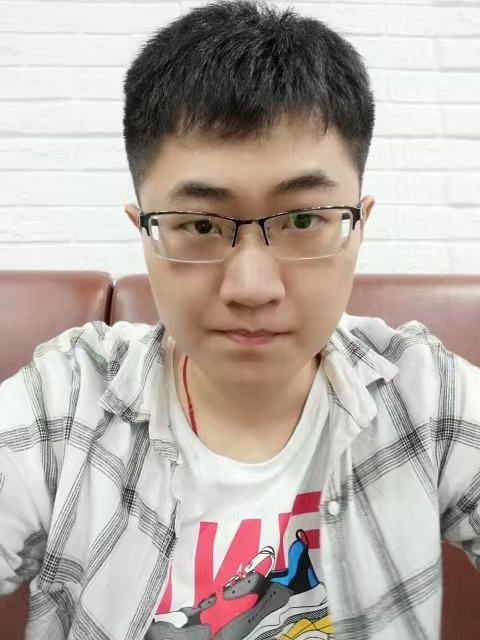
\includegraphics[width=0.15\textwidth]{photo}
	%\end{wrapfigure}
	{\centering{ \Huge \usefont{OT1}{phv}{b}{n} {Xu Du}}
		\par \normalsize \normalfont}
	%\MyName{Xu Du}
	%\MySlogan{Nombre de tu carrera}
	
	%\sepspace
	
	%%% Personal details
	%%% ------------------------------------------------------------
	\NewPart{CONTACT INFO}{}
	
	\PersonalEntry{Address:}{N0.266-38 Mingli Road, Zhengzhou, Henan, P.R.China}
	%\PersonalEntry{Address}{111 First St, New York}
	\PersonalEntry{Website:}{https://fubianhanshu9.github.io/index.html}
	\PersonalEntry{E--Mail:}{\url{duxu@hnas.ac.cn}}%{\url{duxu@shanghaitech.edu.cn}}
	
	%%% Education
	%%% ------------------------------------------------------------
	\NewPart{EXPERIENCE}
	\begin{itemize}
		\item Postdoctoral Researcher, National Key Laboratory of Science and Technology on Communications,  University of Electronic Science and Technology of China, 2023.1-2023.6.
	\end{itemize}
	
	%\textbf{Boris Houska}
	\NewPart{EDUCATION}{}
	
	\EducationEntry{University of Chinese Academy of Sciences\\Shanghai Institute of Microsystem and Information Technology, Chinese Academy of Sciences}{Sep.2017-Sep.2022}{Ph.D.  in Electrical Engineering (Supervised by Professor Boris Houska)}
	%{\begin{itemize}
			%\item{Especialidad }
			%\item{Asignaturas más relevantes de carrera/especialidad}
			%\item{Proyecto de fin de carrera: \emph{título del proyecto}}
			%\end{itemize}
			%}
		
		\sepspace
		
		\EducationEntry{Zhengzhou  University}{Sep.2013-June.2017}{B.E,Computer Science, School of Information Engineering  }
		
		%%% Work experience
		%%% ------------------------------------------------------------
		\NewPart{RESEARCH INTERESTS}{}
		%\EducationEntry{Power System State Estimation}
		\begin{itemize}
			
			\item{Distributed Optimization}
			\item{Optimal Experiment Design}
			
			
			
			\item{Algorithmic Game Theory}
			
			\item{Robust Optimization}
			
			\item{Power Systems}
			%	
			\item{Wireless Communication}
		\end{itemize}
		
		
		\NewPart{PUBLICATION}{}
		$\dag$:  equal contribution
		%\textbf{Conference Paper}
		%\EducationEntry{Power System State Estimation}
		%\section{Conference}
		\begin{itemize}
			\item  { \textbf{Xu Du}, Jingzhe Wang. \\
				{Consensus ALADIN: A Framework for
					Distributed Optimization and Its Application in
					Federated Learning}\\
				\emph{ Submit to IEEE Transactions on Pattern Analysis and Machine Intelligence
			} }
			
			
			\item  { \textbf{Xu Du}$^{\dag}$, Shijie Zhu$^{\dag}$, Yifei Wang$^{\dag}$, Boyu Han$^{\dag}$, Xiaohe He$^{\dag}$. \\
				{Optimal Resilience Design of AC Microgrid
					using AO-SBQP Method}\\
				\emph{ The 22nd IFAC World Congress, Yokohama, Japan, 2023
			} }
			
			\item  { \textbf{Xu Du}, Alexander Engelmann, Timm Faulwasser, Boris Houska. \\
				{Approximations for Optimal Experimental Design
					in Power System Parameter Estimation (invited session)}\\
				\emph{ The 61th IEEE Conference on Decision and Control (CDC), Canc\'un, Mexico, 2022
			} }
			
			
			\item  { Shijie Zhu$^{\dag}$, \textbf{Xu Du}$^{\dag}$. \\
				{Alternating Direction Based Sequential Boolean Quadratic Programming Method for Transmit Antenna Selection}\\
				\emph{ The 61th IEEE Conference on Decision and Control (CDC), Canc\'un, Mexico, 2022
			} }
			
			\item  { Boyu Han, Xuwen Liang, Zhuochen Xie, \textbf{Xu Du}, Xiaohe He. \\
				{Communication Enhancement Model of Intelligent Reflecting Surface Based on Cooperative Relationship}\\
				\emph{Laser $\&$ Optoelectronics Progress, 2021
			} }
			
			\item  { \textbf{Xu Du}, Alexander Engelmann, Timm Faulwasser, Boris Houska. \\
				{Online power system parameter estimation and optimal operation}\\
				\emph{In Proceedings of the 2021 American Control Conference (ACC), New Orleans, USA May, 2021
			} }
			
			\item  {\textbf{Xu Du}, Alexander Engelmann, Yuning Jiang, Timm Faulwasser, Boris Houska. \\
				Optimal Experiment Design for AC Power Systems Admittance Estimation\\
				\emph{In Proceedings of the 21rst IFAC World Congress, Berlin, Germany, July, 2020
			} }
			
			\item  {\textbf{Xu Du}, Alexander Engelmann, Yuning Jiang, Timm Faulwasser, Boris Houska. \\
				Distributed State Estimation for AC Power Systems using Gauss-Newton ALADIN \\
				\emph{In Proceedings of the 58th IEEE Conference on Decision and Control (CDC),
					Nice, France, December, 2019.} }
			%\item{Optimal Experimental Design}
			%\item{Función 3}
		\end{itemize}
		%\textbf{Journal Article }
		%\section{Journal}
		
		\NewPart{Professional Service}{Conference Session Chair/Co-chair}
		%
		%\EducationEntry{Título trabajo 1}{Periodo}{Empresa}{
			\begin{itemize}
				\item{Co-chair of the invited session for the 61st
					IEEE Conference on Decision and Control (CDC 2022)
					“Trends in Optimization for Power Systems”, Canc\'un, Mexico} (together with Alexander Engelmann, Timm Faulwasser, Boris Houska)
			\end{itemize}
			{Technical Meetings—Leadership Roles}
			\begin{itemize}
				\item{Co-organizer, International Workshop on Advanced Methods for Control and Estimation of Dynamic
					Systems (AMCEDS 2018), ShanghaiTech University, Shanghai, China, July 23, 2018}
				%\item{Función 2}
				%\item{Función 3}
			\end{itemize}
			{Technical Reviewer}
			\begin{itemize}
				\item Selected journals: Optimal Control Applications $\&$ Methods
				\item Selected international conferences: CDC, IFAC World Congress, ICCA
			\end{itemize}
			
			\NewPart{PRESENTATION}{}
			\begin{itemize}
				\item {
					{Sub-linear Convergence of ADMM}\\
					\emph{ShanghaiTech, China, December 8th, 2022 (Online)	} }
				
				
				\item  {
					{Distributed Optimization with ADMM and	ALADIN}\\
					\emph{Innovation Academy for Microsatellite, Chinese Academy of Sciences, China, November, 2021 	} }
				\item  {
					{Online power system parameter estimation and optimal operation}\\
					\emph{2021 American Control Conference (ACC), New Orleans, USA May, 2021 (online)
				} }
				
				\item  {
					Optimal Experiment Design for AC Power Systems Admittance Estimation\\
					\emph{21rst IFAC World Congress, Berlin, Germany, July, 2020 (online)
				} }
				
				\item  {
					Distributed State Estimation for AC Power Systems using Gauss-Newton ALADIN 
					\emph{58th IEEE Conference on Decision and Control (CDC),
						Nice, France, December, 2019.} }
			\end{itemize}
			
			
			\NewPart{HONORS AND AWARDS}
			\begin{itemize}
				\item Merit Student, ShanghaiTech University, 2019-2020
				
				\item SIST Outstanding Teaching Assistant Award, ShanghaiTech University, 2019-2020
				
				%\item SIST Outstanding Teaching Assistant Award, ShanghaiTech University, 2019
				
				\item Outstanding Student Award, Zhengzhou University, 2014-2017
				
				\item YiSheng Scholarship, Zhengzhou University, 2015
				
				
			\end{itemize}
			%\sepspace
			%
			%\EducationEntry{Título trabajo 2}{Periodo}{Empresa}{Descripción, habilidades}
			\NewPart{URL Links}
			\begin{itemize}
				\item Google Scholar: \url{https://scholar.google.com/citations?user=OnIuCR0AAAAJ}
				\item ResearchGate: \url{https://www.researchgate.net/profile/Xu-Du-9}
				\item ORCID \url{https://orcid.org/my-orcid?orcid=0009-0007-6789-1222}
			\end{itemize}
			\NewPart{Advising}{Co-supervised Students}
			\begin{itemize}
				\item Co-supervisor of Boyu Han, Innovation Academy for Microsatellite, Chinese Academy of Sciences, 2021.
				(Master 2021, now Ph.D in Shanghai Jiaotong University)
				\item Co-supervisor of Shijie Zhu, Innovation Academy for Microsatellite, Chinese Academy of Sciences, 2021-2023.
				(Master 2023, now with China Telecom)
				\item Co-supervisor of Yifei Wang, Innovation Academy for Microsatellite, Chinese Academy of Sciences, 2021-2023.
				(Master 2023)
			\end{itemize}
			
			\NewPart{Teaching}{ShanghaiTech}
			\begin{itemize}
				
				
				\item{Teaching Assistant, 	Introduction to Communication Systems (EE140), ShanghaiTech University, Fall 2021 (Instructor: Professor Lixiang Lian).}
				
				\item{Teaching Assistant, Signals and Systems Lab(EE150L), ShanghaiTech University, Spring 2021 (Instructor: Linyan Lu and Ping Wang).}
				
				\item{Teaching Assistant, Introduction to Control(EE160), ShanghaiTech University, Fall 2020\\ 
					http://faculty.sist.shanghaitech.edu.cn/faculty/boris/EE160.html\\
					(Instructor: Professor Boris Houska and Professor Yang Wang).
				}
				
				\item{Teaching Assistant, Introduction to Control Project(EE160P), ShanghaiTech University, Fall 2020\\ (Instructor: Professor Boris Houska and Professor Yang Wang).}
				
				\item{Teaching Assistant, Signals and Systems(EE150),  ShanghaiTech University, Spring 2020 \\ (Instructor: Professor Yong Zhou, Professor Ziping Zhao, Professor Xin Lou and Professor Lin Xu).}
				
				\item{Teaching Assistant, Numerical Analysis(SI211), ShanghaiTech University, Fall 2019\\ 
					{http://faculty.sist.shanghaitech.edu.cn/faculty/boris/SI211.html}\\
					(Instructor: Professor Boris Houska).
				}
				
				\item{Teaching Assistant, Design Thinking, ShanghaiTech University, Fall 2018 and Spring 2019.\\ (Instructor: Professor Ding Lu, Professor Xiyi Yang and Professor Xue Chen) }
				
				\item{Teaching Assistant, Signals and Systems(EE150),  ShanghaiTech University, Spring 2018 (Instructor: Professor Yanlin Geng)
					
				}
				%	\item{Teaching Assistant, Design Thinking, ShanghaiTech University, Fall 2018.}
				%	\item{Teaching Assistant, Signals and Systems,  ShanghaiTech University, Spring 2018}
				
				
				
			\end{itemize}
			%\SkillsEntry{}{}
			
			
			
			
			%%% References
			%%% ------------------------------------------------------------
			%\NewPart{References}{}
			%Available upon request
		\end{document}